%presentation declaration
\documentclass[10pt]{beamer}
\usetheme{metropolis}

%packages
%beamer stuff
\usepackage{appendixnumberbeamer}
\usepackage{booktabs}
\usepackage[scale=2]{ccicons}
\usepackage{pgfplots}
\usepgfplotslibrary{dateplot}
\usepackage{xspace}
%language
\usepackage[brazilian]{babel}
\usepackage[utf8]{inputenc}
%images
\usepackage{graphicx}
\usepackage{float}

%macros
\newcommand{\tit}[1]{\textit{#1}}
\newcommand{\tbf}[1]{\textbf{#1}}
\newcommand{\ttt}[1]{\texttt{#1}}

%title
\title{Atenção Visual Eficiente com Deep Learning}
\subtitle{}
\author{Erik Perillo, Esther Colombini}
\date{}
\institute{Instituto de Computação -- Unicamp}

\begin{document}

\maketitle

\section{Visão}

\begin{frame}{}
    \begin{figure}
        \centering
        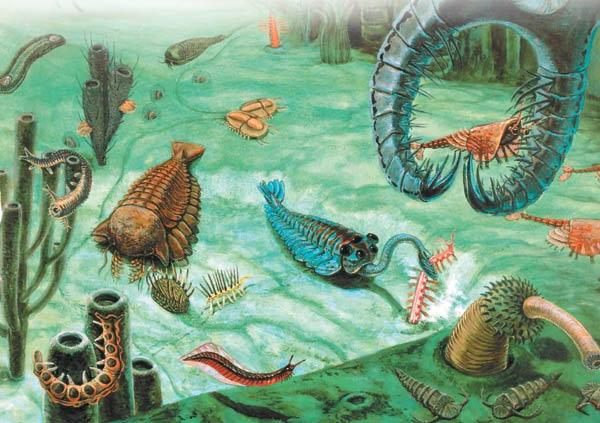
\includegraphics[width=1.0\linewidth]{./img/precambrian}
    \end{figure}
\end{frame}

\begin{frame}{}
    \begin{figure}
        \centering
        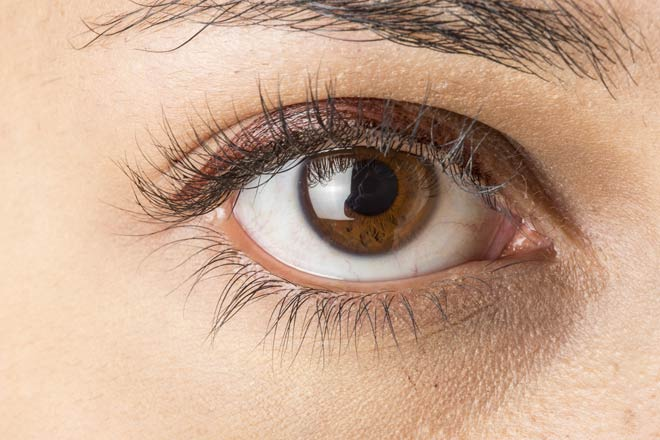
\includegraphics[width=1.0\linewidth]{./img/eye.jpg}
    \end{figure}
\end{frame}

%\begin{frame}{}
%    \begin{figure}
%        \centering
%        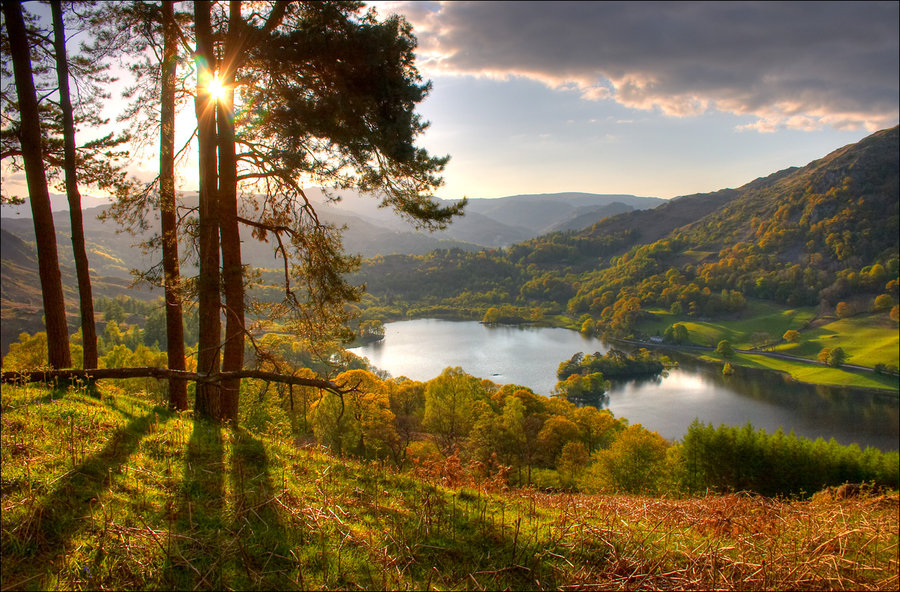
\includegraphics[width=1.0\linewidth]{./img/beautiful_landscape.jpg}
%    \end{figure}
%\end{frame}

\begin{frame}{}
    \begin{figure}
        \centering
        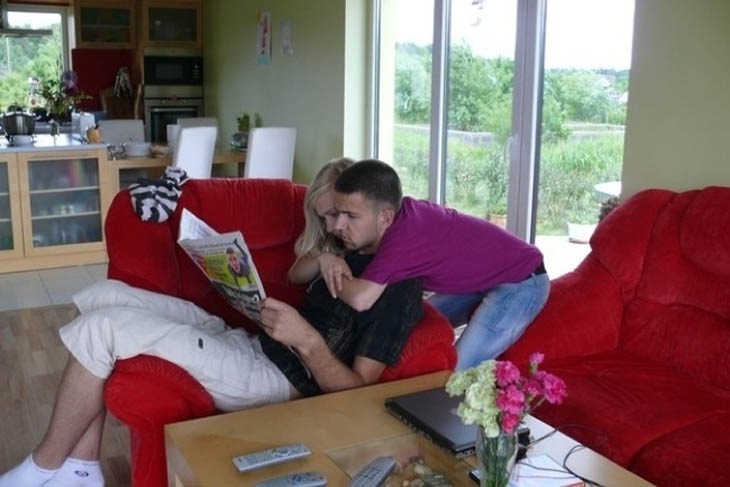
\includegraphics[width=1.0\linewidth]{./img/confusing_image_4.jpg}
    \end{figure}
\end{frame}

\begin{frame}{}
    \begin{figure}
        \centering
        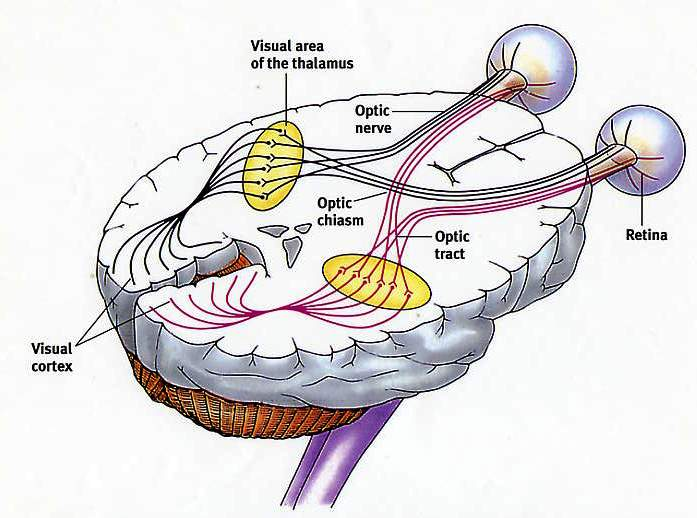
\includegraphics[width=0.9\linewidth]{./img/visual_system_brain.jpg}
    \end{figure}
\end{frame}

\begin{frame}{}
    \begin{figure}
        \centering
        
\includegraphics[width=0.9\linewidth]{./img/wheres_wally.jpg}
    \end{figure}
\end{frame}

\begin{frame}{}
    \begin{figure}
        \centering
        
\includegraphics[width=0.9\linewidth]{./img/wheres_wally_focus_1.jpg}
    \end{figure}
\end{frame}

\begin{frame}{}
    \begin{figure}
        \centering
        
\includegraphics[width=0.9\linewidth]{./img/wheres_wally_focus_2.jpg}
    \end{figure}
\end{frame}

\begin{frame}{Atenção Visual}
    \begin{quote}
        Seleção de uma certa região espacial do campo visual para
        posterior processamento cognitivo
    \end{quote}
\end{frame}

\begin{frame}{Atenção: Top-down versus Bottom-up}
    \begin{itemize}[<+->]
        \item Top-down: Estímulo interno do ser que direciona a atenção
            a padrões específicos de estímulo visual
        \item \tbf{Bottom-up (saliência visual):}
            Estímulo externo que capta a atenção visual
    \end{itemize}
\end{frame}

\begin{frame}{}
    \begin{figure}
        \centering
        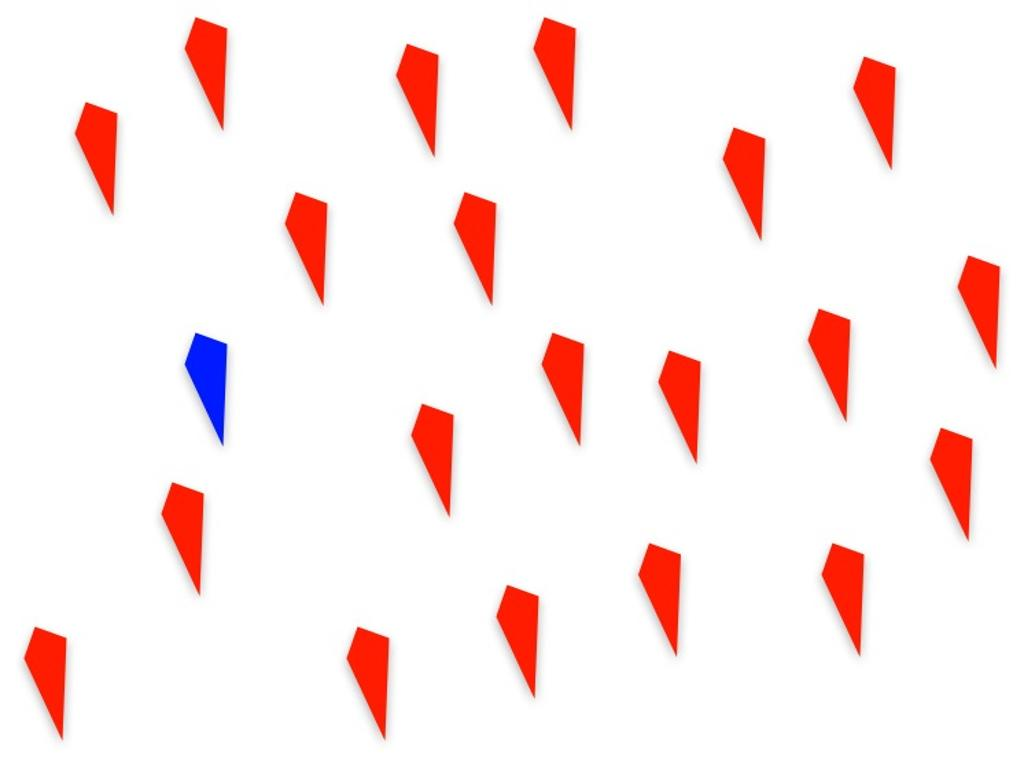
\includegraphics[width=0.8\linewidth]{./img/syntheticData2.jpg}
    \end{figure}
\end{frame}

\begin{frame}{}
    \begin{figure}
        \centering
        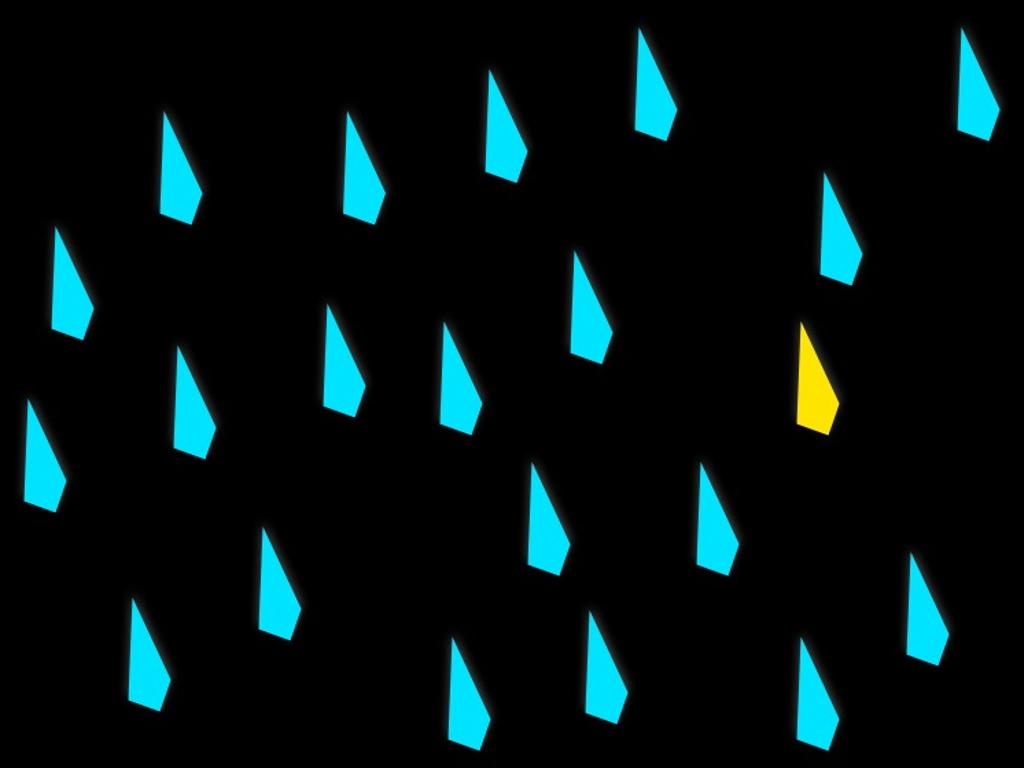
\includegraphics[width=0.8\linewidth]{./img/syntheticData5.jpg}
    \end{figure}
\end{frame}

\begin{frame}{}
    \begin{figure}
        \centering
        
\includegraphics[width=0.8\linewidth]{./img/syntheticData1.jpg}
    \end{figure}
\end{frame}

\begin{frame}{}
    \begin{figure}
        \centering
        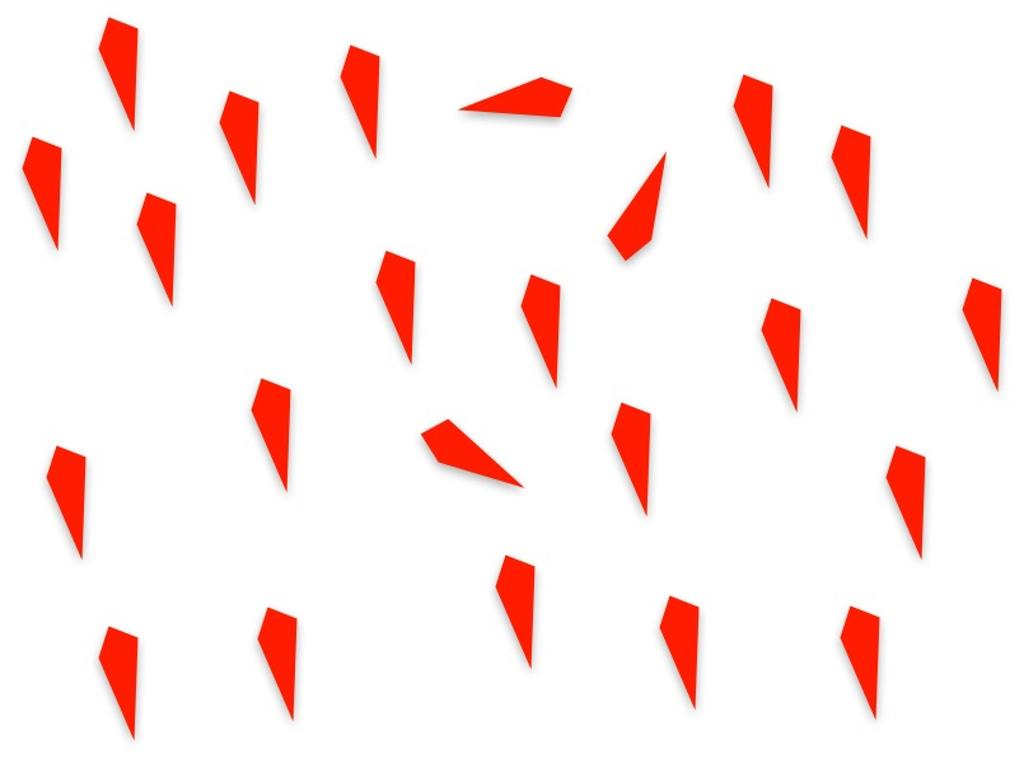
\includegraphics[width=0.8\linewidth]{./img/syntheticData3.jpg}
    \end{figure}
\end{frame}

\begin{frame}{}
    \begin{figure}
        \centering
        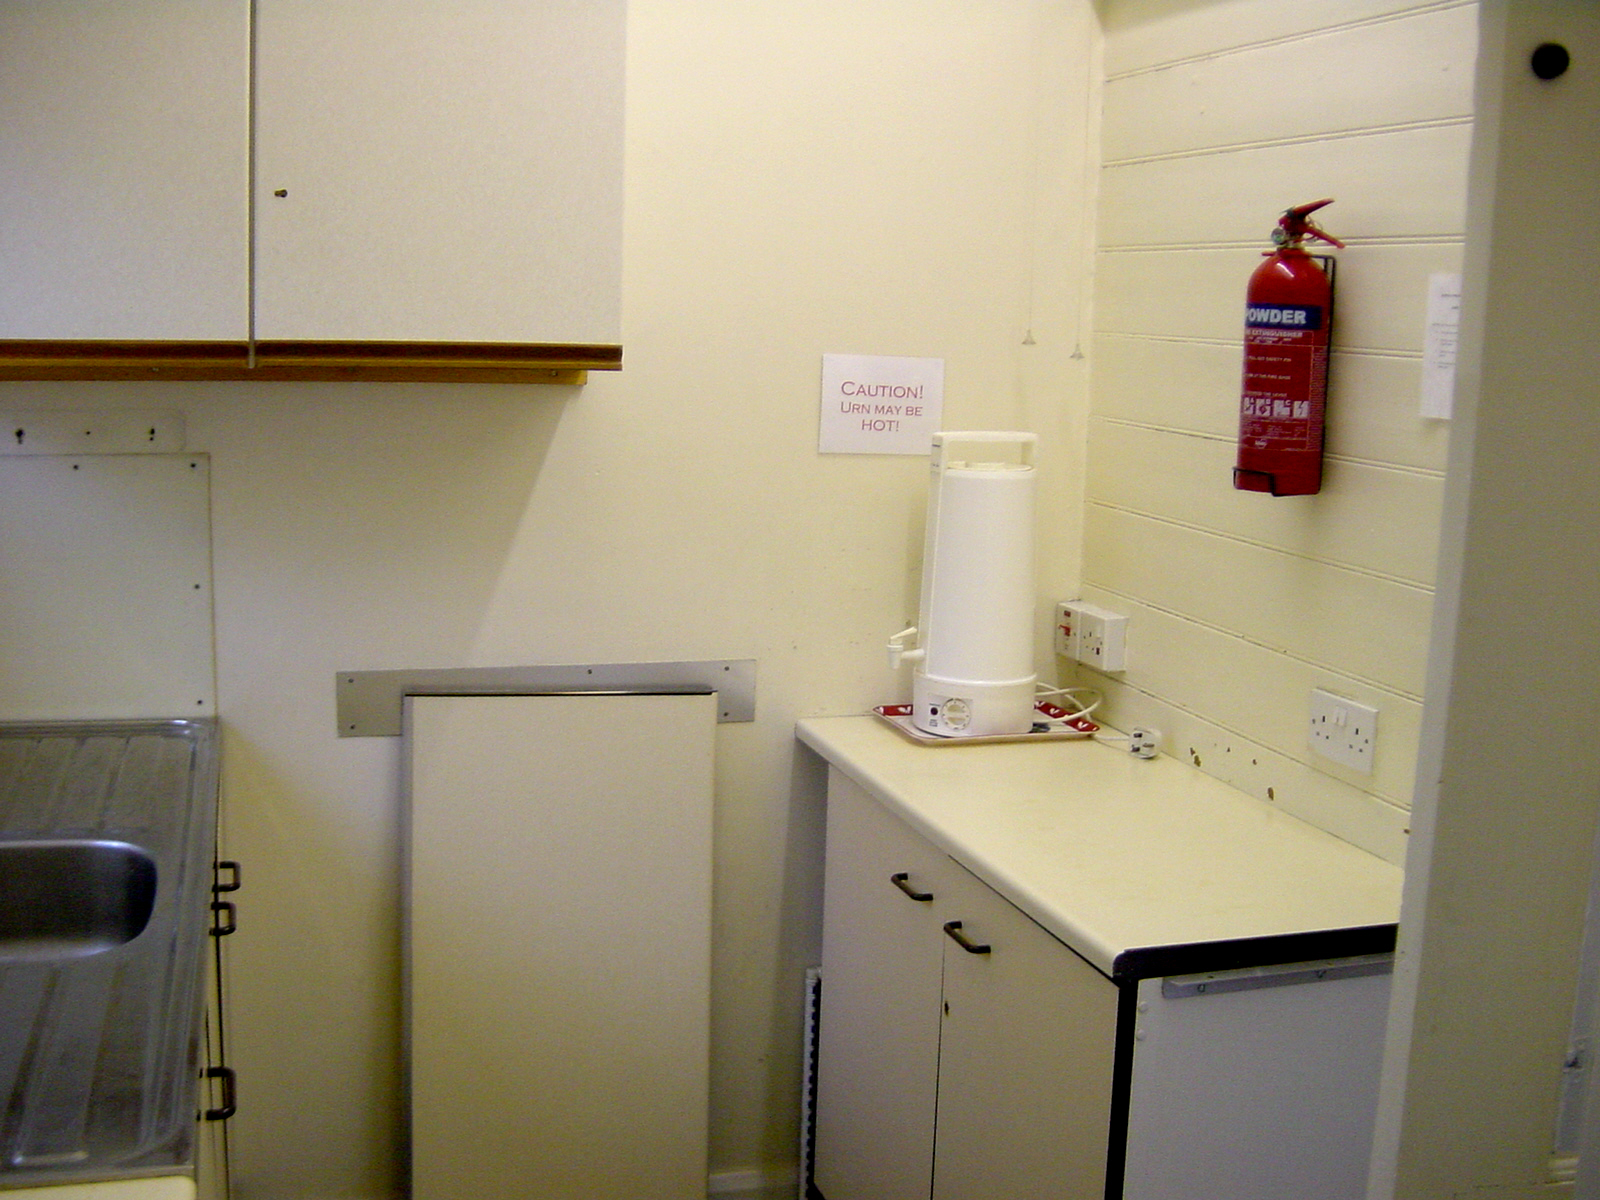
\includegraphics[width=0.9\linewidth]{./img/fire_extinguisher.jpg}
    \end{figure}
\end{frame}

\begin{frame}{Mapa de saliência}
    \begin{figure}
        \centering
        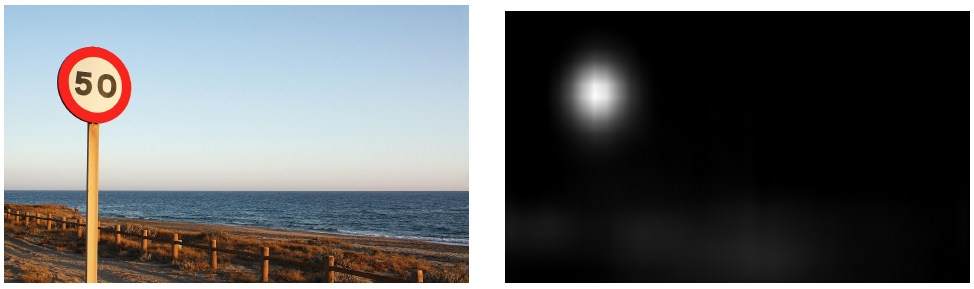
\includegraphics[width=1.0\linewidth]{./img/saliency_map_ex_1.png}
    \end{figure}
\end{frame}

\begin{frame}{}
    \begin{center}
        \begin{tabular} {cc}
        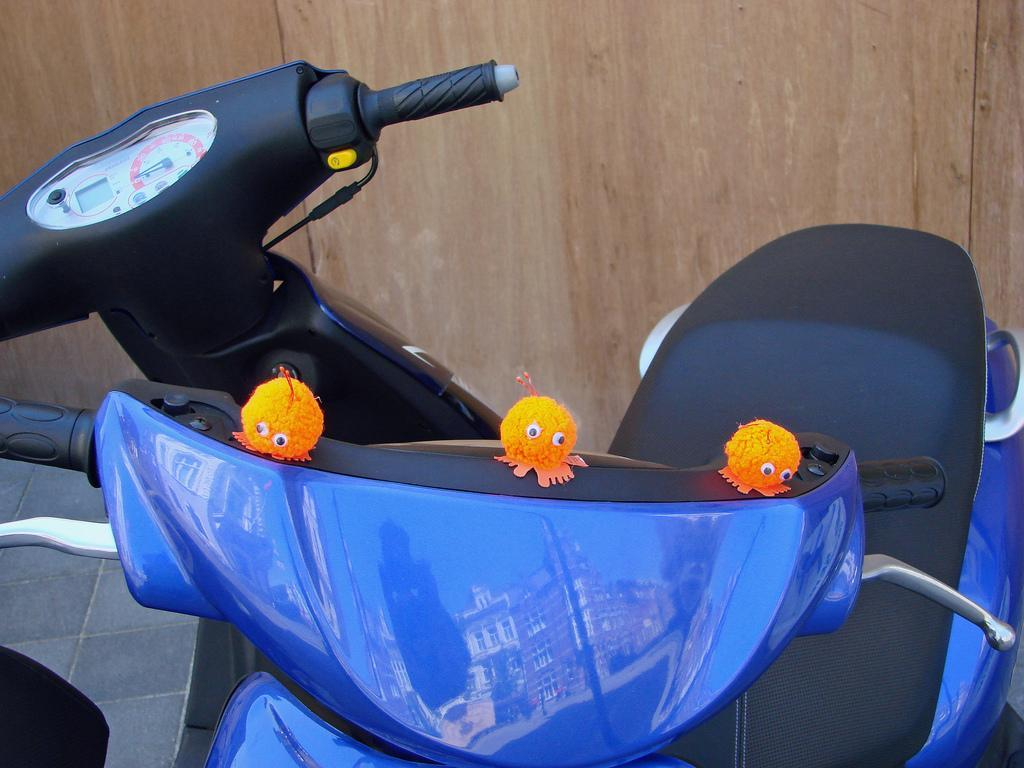
\includegraphics[width=0.45\textwidth]{./img/orange_balls.jpg} &
        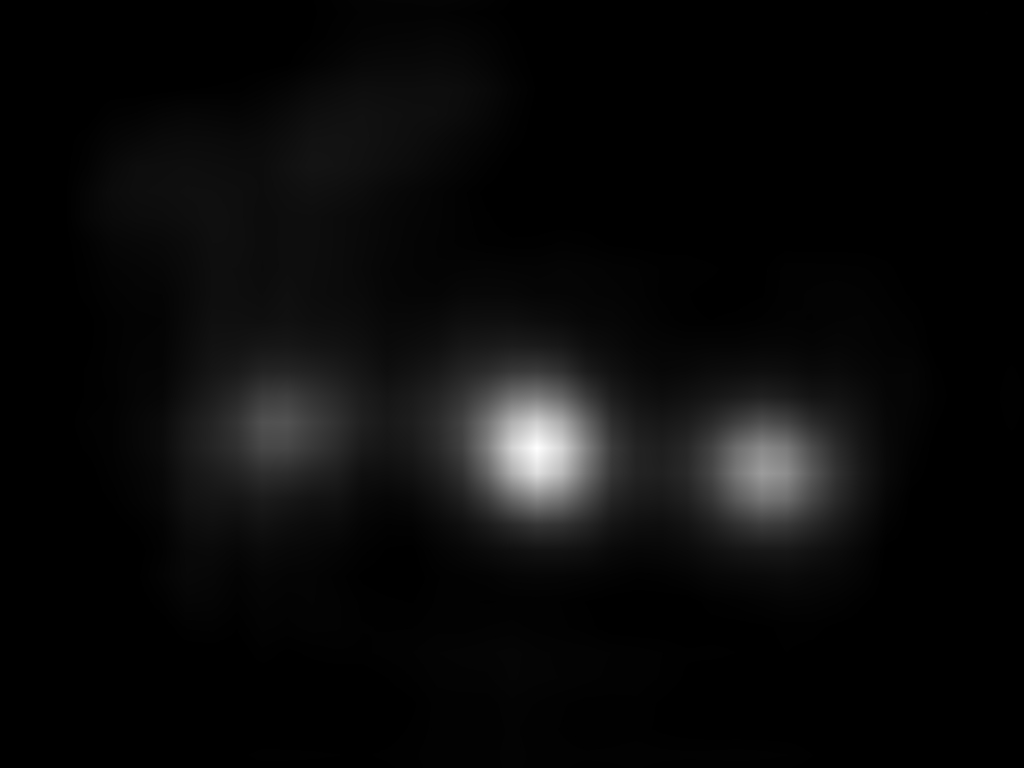
\includegraphics[width=0.45\textwidth]{./img/orange_balls_map.jpg}
        \end{tabular}
    \end{center}
\end{frame}

\begin{frame}{}
    \begin{center}
        \begin{tabular} {cc}
        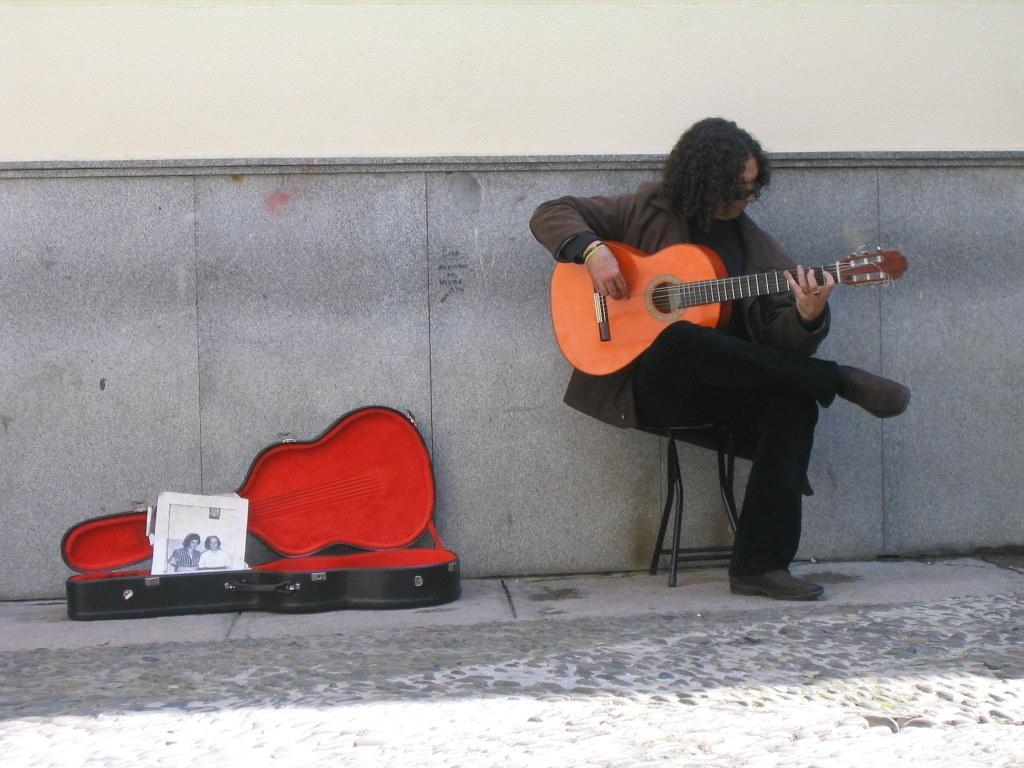
\includegraphics[width=0.45\textwidth]{./img/guitarist.jpg} &
        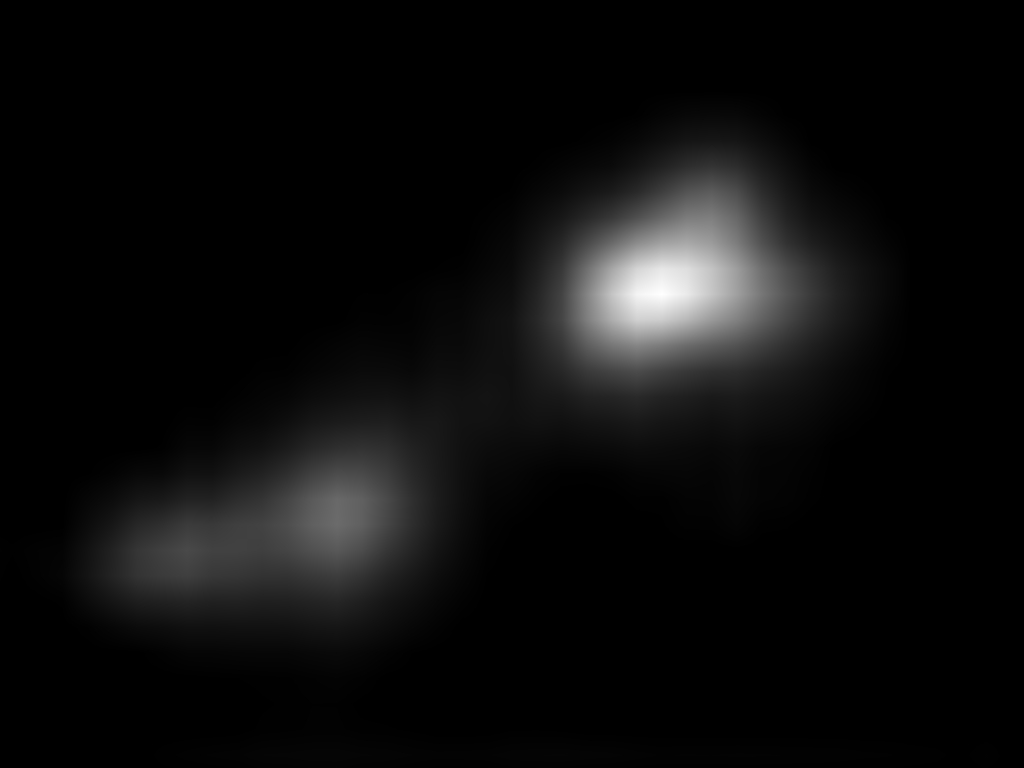
\includegraphics[width=0.45\textwidth]{./img/guitarist_map.jpg}
        \end{tabular}
    \end{center}
\end{frame}

\begin{frame}{}
    \begin{center}
        \begin{tabular} {cc}
        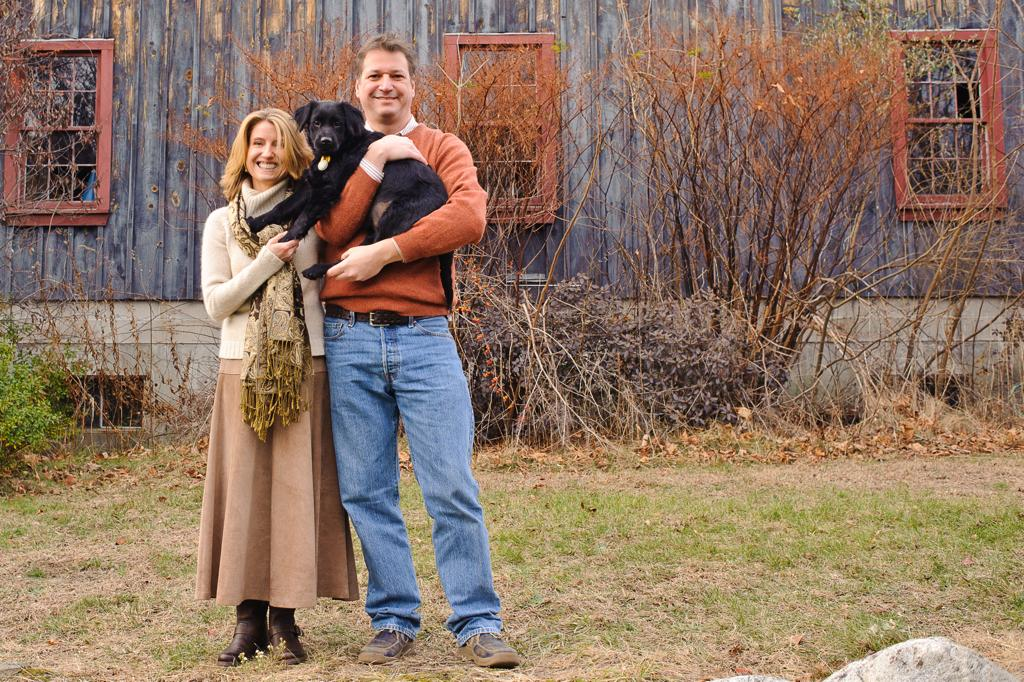
\includegraphics[width=0.45\textwidth]{./img/couple.jpg} &
        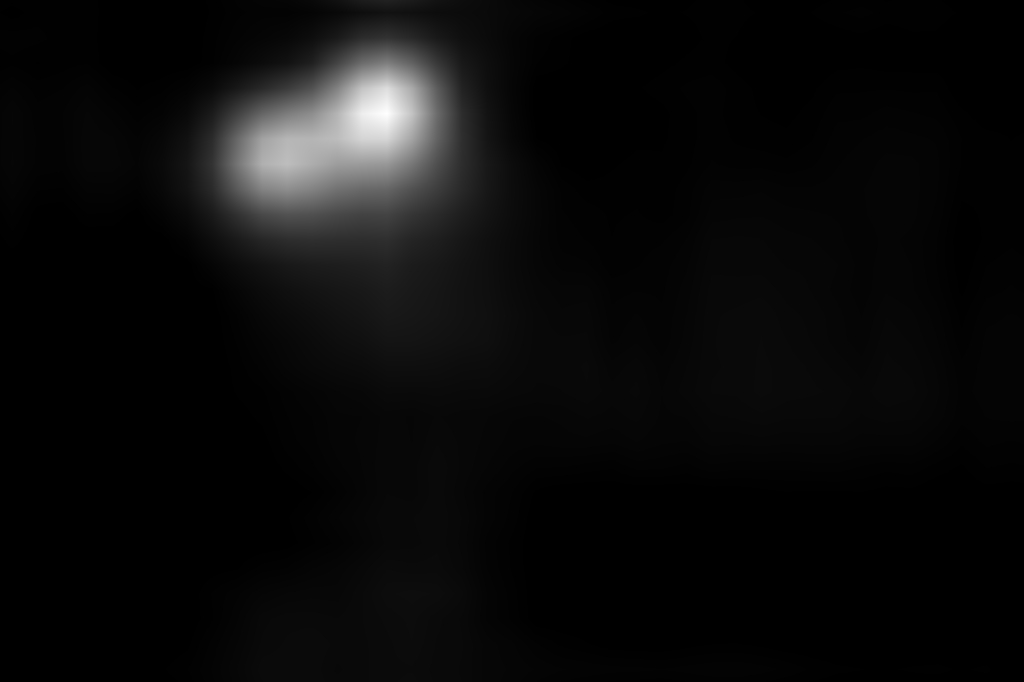
\includegraphics[width=0.45\textwidth]{./img/couple_map.jpg}
        \end{tabular}
    \end{center}
\end{frame}

\begin{frame}{}
    \begin{quote}
        Podemos fazer um computador identificar saliências visuais?
    \end{quote}
\end{frame}

\begin{frame}{Modelo de saliência visual}
    \tbf{Ideia:}
    \begin{itemize}[<+->]
        \item Dada uma imagem, gerar um mapa de saliência coerente
            com o que humanos gerariam
    \end{itemize}
\end{frame}

\begin{frame}{Modelo de saliência visual}
    \tbf{Problemas:}
    \begin{itemize}[<+->]
        \item Saliência emerge de relações muito complexas em imagens normais
        \item É difícil captar todas as nuances envolvidas apenas extraindo
            \tit{features} pré-determinadas
    \end{itemize}
\end{frame}

\begin{frame}{}
    \begin{center}
        \begin{tabular} {cc}
        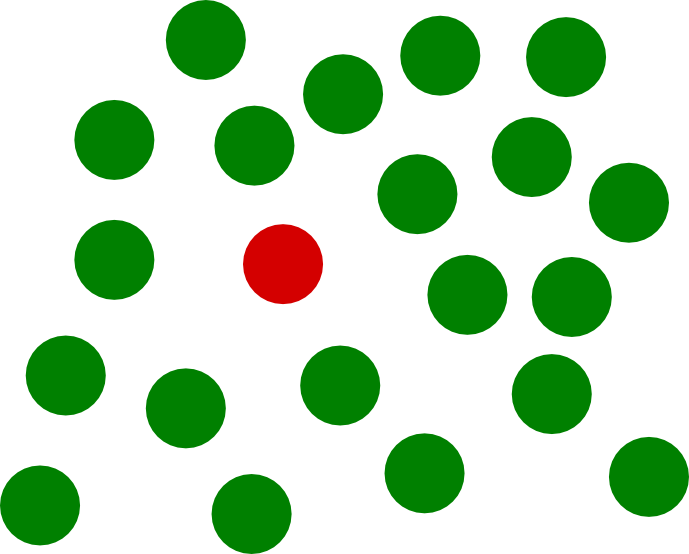
\includegraphics[width=0.45\textwidth]{./img/red_in_green.png} &
        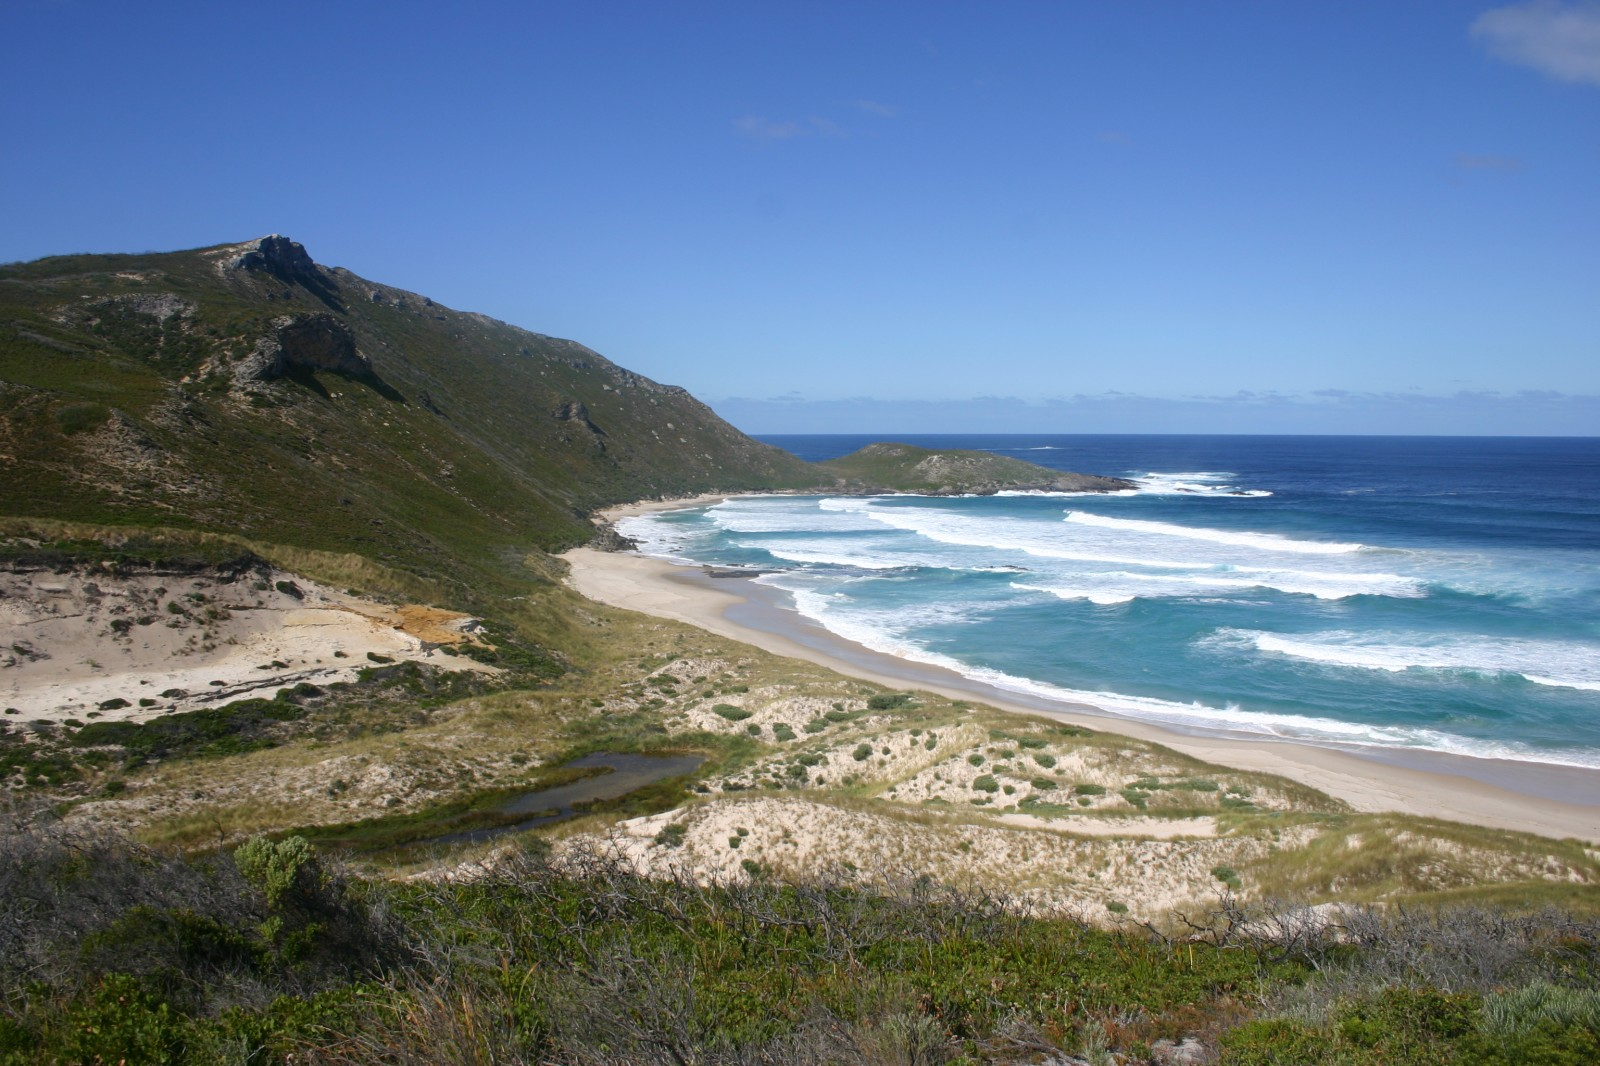
\includegraphics[width=0.45\textwidth]{./img/cliff.jpg}
        \end{tabular}
    \end{center}
\end{frame}

\begin{frame}{Deep Learning}
    \begin{center}
        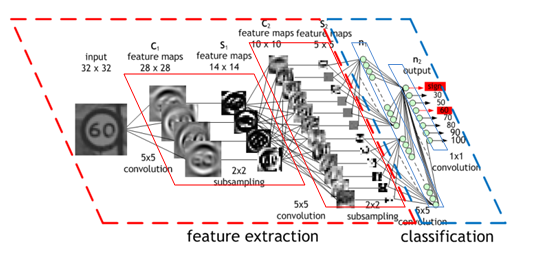
\includegraphics[width=1.0\textwidth]{./img/convnet.png}
    \end{center}
\end{frame}

\begin{frame}{VGG-16}
    \begin{center}
        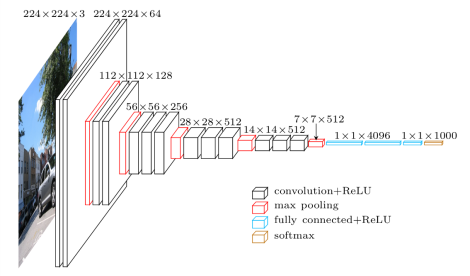
\includegraphics[width=0.8\textwidth]{./img/vgg16.png}
    \end{center}
\end{frame}

\section{Objetivo}

\begin{frame}{}
    \begin{quote}
        É possível um modelo de saliência visual que seja \tbf{efetivo} e
        mais \tbf{computacionalmente eficiente}?
    \end{quote}
\end{frame}

\section{Modelo Proposto}

\begin{frame}{Hipótese: aspectos relevantes}
    \begin{itemize}[<+->]
        \item Rede neural totalmente convolucional específica para saliência
        \item Arquitetura que extraia informações de contraste e
            múltiplas dimensões
        \item Pré-processamento de dados adequado ao contexto de saliência
            visual
    \end{itemize}
\end{frame}

\begin{frame}{Arquitetura da rede}
    \begin{figure}[hbt]
        \centering
        \def\svgwidth{1.0\columnwidth}
        \input{./img/model.pdf_tex}
        \label{fig:model}
    \end{figure}
\end{frame}

\begin{frame}{Arquitetura da rede}
    \begin{figure}[hbt]
        \centering
        \def\svgwidth{1.0\columnwidth}
        \input{./img/model.pdf_tex}
        \label{fig:model}
    \end{figure}
    \begin{itemize}[<+->]
        \item Entrada: (H x W x 3)
        \item \tbf{1.} Convolução/ReLU + MaxPool (H x W x 3)
        \item \tbf{2.} 2 Convoluções/ReLU + MaxPool (H/2 x W/2 x 48)
        \item \tbf{3.} 4 Convoluções/ReLU + MaxPool (H/4 x W/4 x 96)
        \item \tbf{4.} 8 \tit{inception layers} (H/8 x W/8 x 144)
        \item Saída (H/8 x W/8 x 1)
    \end{itemize}
\end{frame}

\begin{frame}{Inception}
    \begin{figure}[hbt]
        \centering
        \def\svgwidth{0.9\columnwidth}
        \input{./img/inception.pdf_tex}
        \label{fig:inception}
    \end{figure}
\end{frame}

\begin{frame}{Pré-processamento de dados}
    \begin{itemize}[<+->]
        \item Espaço de cor \tbf{LAB} ao invés de RGB
        \item Normalização de canais \tbf{por imagem} ao invés de pelo
            \tit{dataset}
    \end{itemize}
\end{frame}

\begin{frame}{Treinamento: Datasets}
    \begin{itemize}[<+->]
        \item Salicon: 15000 imagens
        \item Judd: 1003 imagens
            \tit{dataset}
        \item Aumento de dados por espelhamento de imagem
    \end{enumerate}
\end{frame}

\begin{frame}{Treinamento: Função objetivo}
    \begin{center}
        $$min~ CC(P, T) = \frac{cov(P, T)}{\sigma(P)\sigma(T)}$$
    \end{center}
\end{frame}

\begin{frame}{Treinamento: Função objetivo}
    \begin{center}
        $$min~ CC(P, T) = \frac{cov(P, T)}{\sigma(P)\sigma(T)}$$
    \end{center}
    \begin{itemize}[<+->]
        \item Penalização equilibrada de falsos positivos/negativos
        \item Não força a rede a produzir valores em uma certa escala
    \end{itemize}
\end{frame}

\begin{frame}{Treinamento: Etapa 1}
    \begin{itemize}[<+->]
        \item 30000 imagens advindas do Salicon
        \item \tit{SGD} + \tit{Nesterov Momentum} de $0.9$
        \item \tit{Learning Rate}: 0.009 por 5 \tit{epochs},
            0.001 por 3 \tit{epochs}
        \item \tit{Batch size}: 10
    \end{enumerate}
\end{frame}

\begin{frame}{Treinamento: Etapa 2}
    \begin{itemize}[<+->]
        \item 2006 imagens advindas do Judd
        \item \tit{SGD} + \tit{Nesterov Momentum} de $0.9$
        \item \tit{Learning Rate}: $5\times 10^{-5}$ por 2 \tit{epochs}
        \item Regularização L2 de $3\times 10^{-5}$
        \item \tit{Batch size}: 2
    \end{enumerate}
\end{frame}

\section{Resultados}

\begin{frame}{}
    \begin{figure}[hbt]
    \begin{center}
		\begin{tabular} {c}
		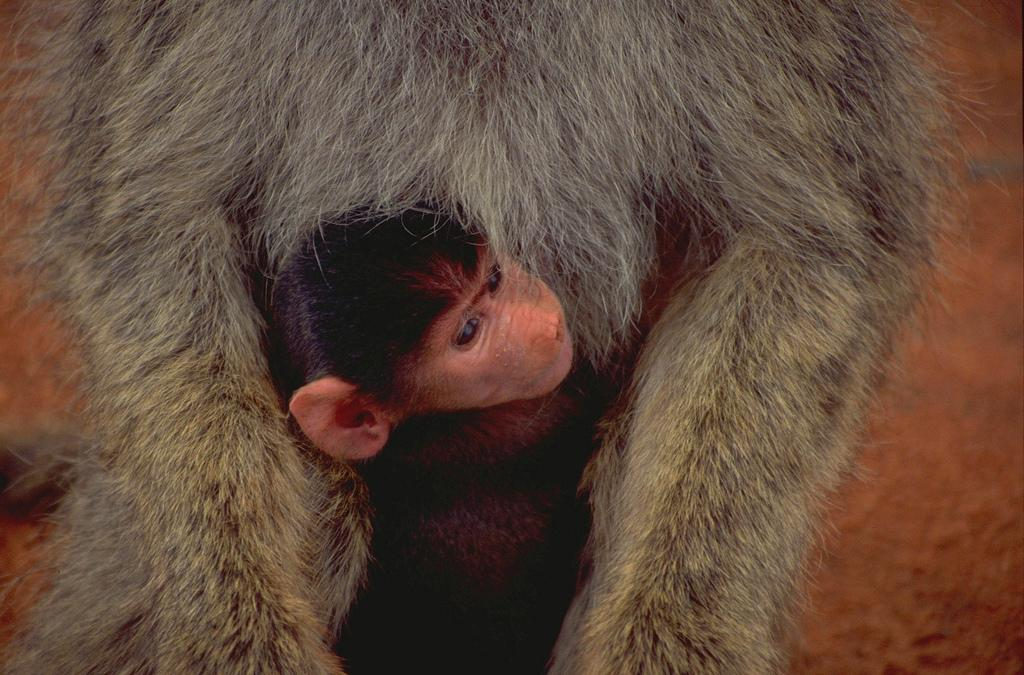
\includegraphics[width=0.33\textwidth]{./img/monkey_s.jpg}
		\end{tabular}
    \end{center}
    \end{figure}
    \begin{figure}[hbt]
    \begin{center}
		\begin{tabular} {cc}
        Humanos & Modelo Proposto\\
        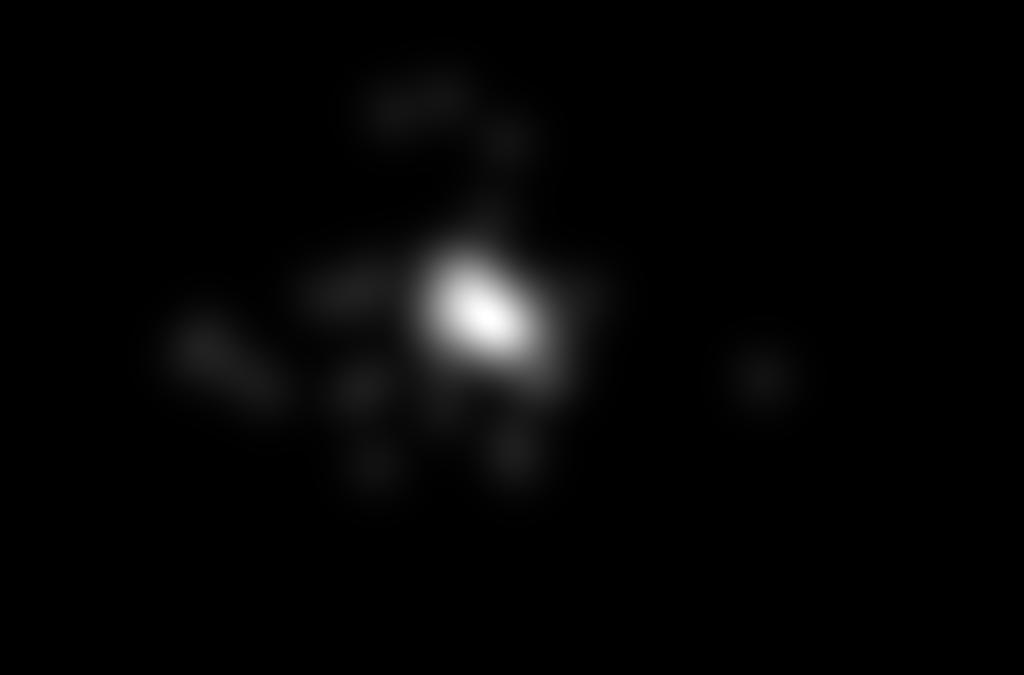
\includegraphics[width=0.33\textwidth]{./img/monkey_gt.jpg} &
		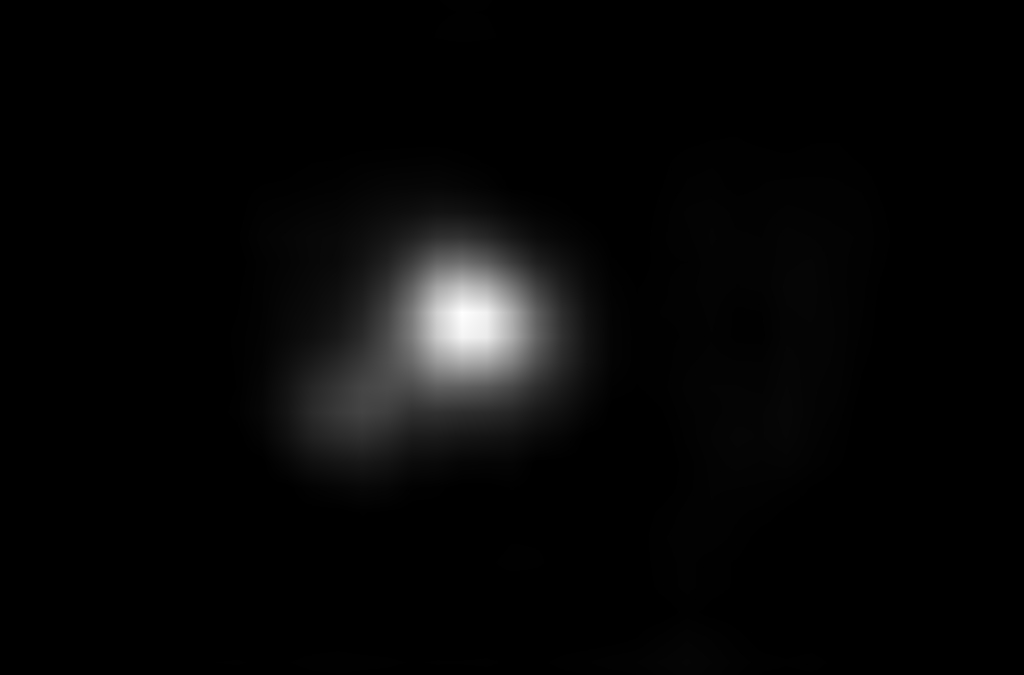
\includegraphics[width=0.33\textwidth]{./img/monkey_m.jpg}
		\end{tabular}
    \end{center}
    \end{figure}
\end{frame}

\begin{frame}{}
    \begin{figure}[hbt]
    \begin{center}
		\begin{tabular} {c}
		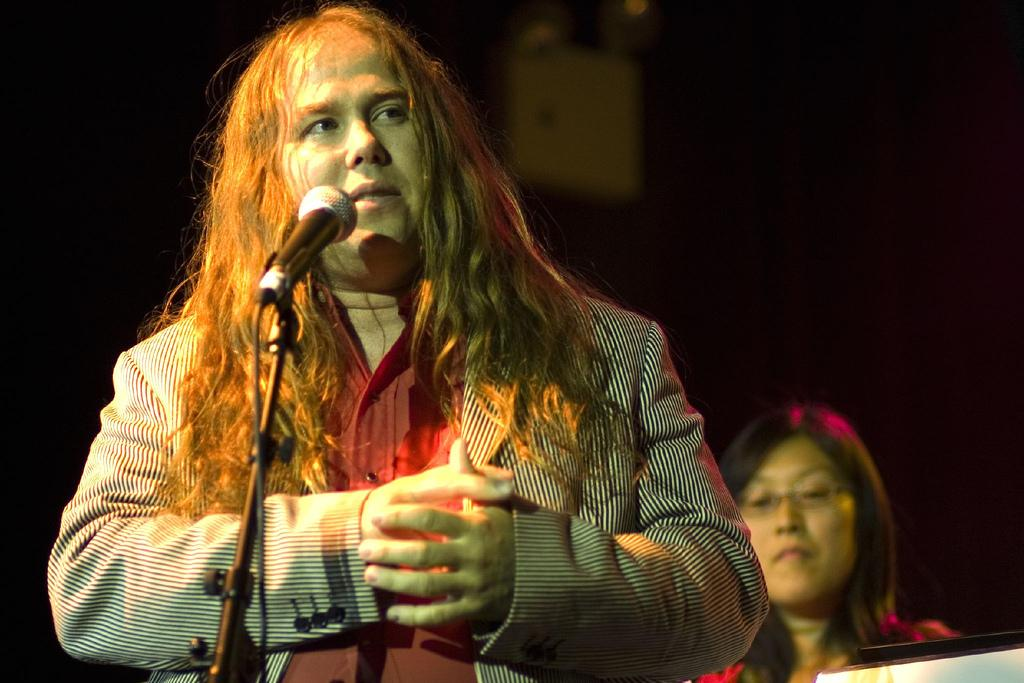
\includegraphics[width=0.33\textwidth]{./img/person_s.jpg}
		\end{tabular}
    \end{center}
    \end{figure}
    \begin{figure}[hbt]
    \begin{center}
		\begin{tabular} {cc}
        Humanos & Modelo Proposto\\
        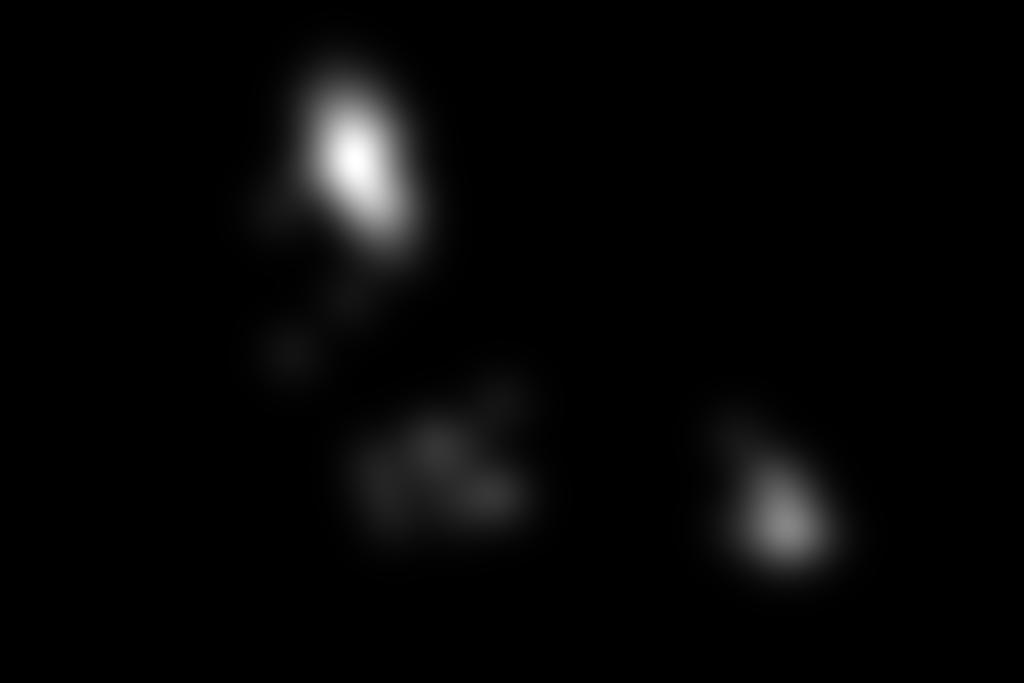
\includegraphics[width=0.33\textwidth]{./img/person_gt.jpg} &
		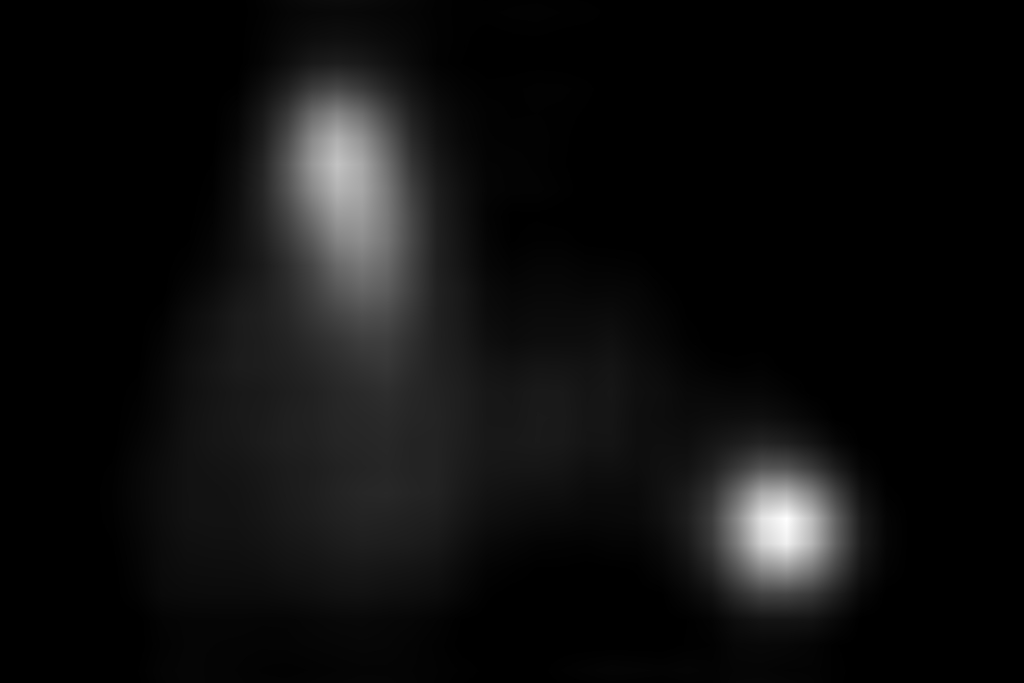
\includegraphics[width=0.33\textwidth]{./img/person_m.jpg}
		\end{tabular}
    \end{center}
    \end{figure}
\end{frame}

\begin{frame}{}
    \begin{figure}[hbt]
    \begin{center}
		\begin{tabular} {c}
		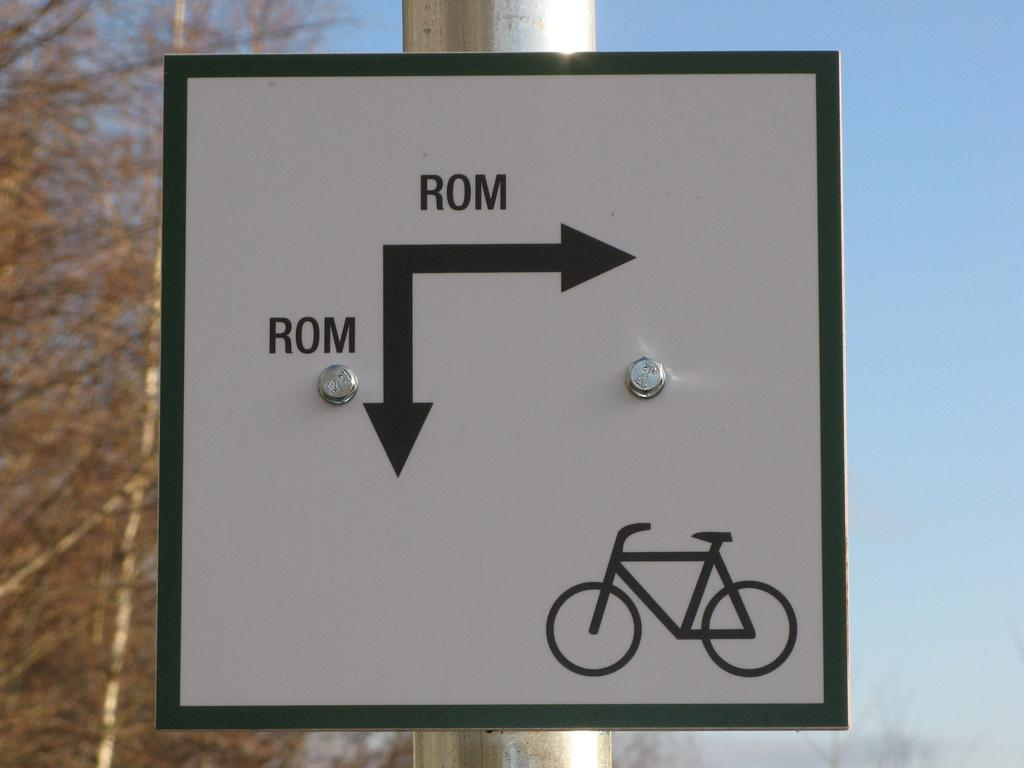
\includegraphics[width=0.33\textwidth]{./img/sign_s.jpg}
		\end{tabular}
    \end{center}
    \end{figure}
    \begin{figure}[hbt]
    \begin{center}
		\begin{tabular} {cc}
        Humanos & Modelo Proposto\\
        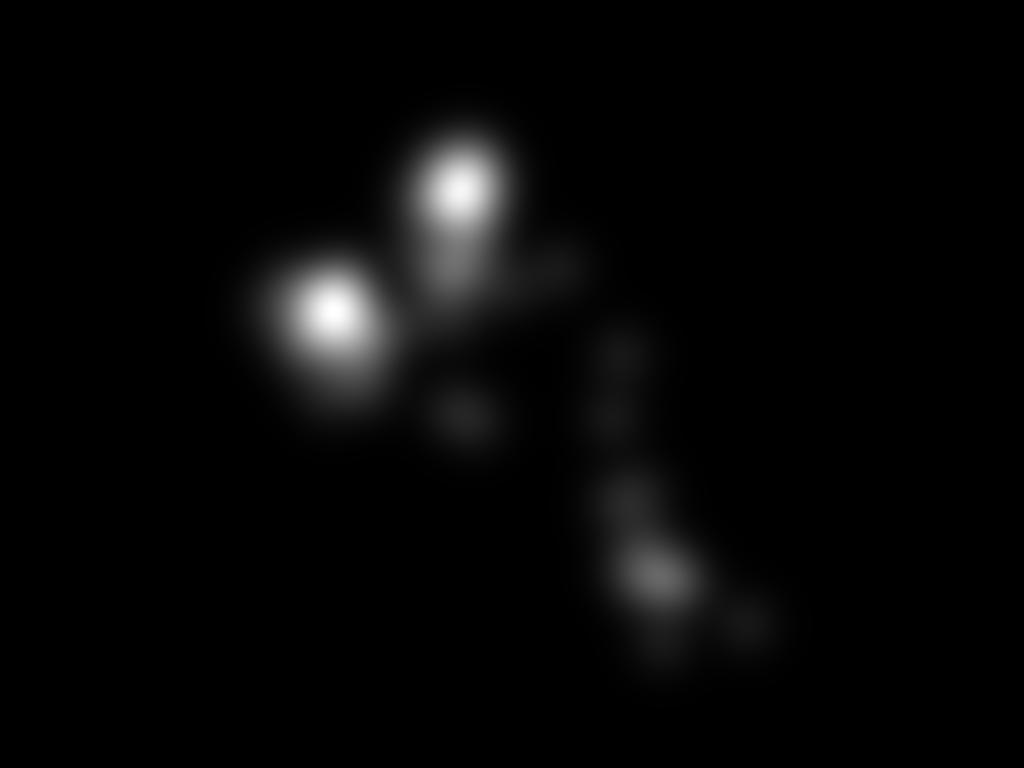
\includegraphics[width=0.33\textwidth]{./img/sign_gt.jpg} &
		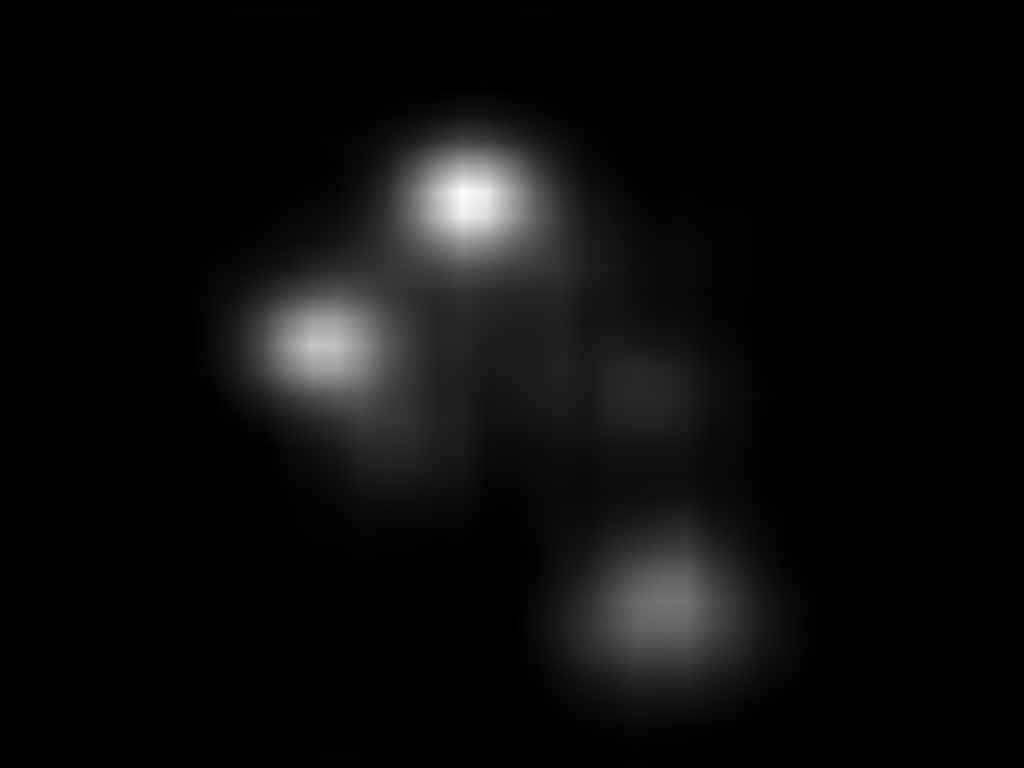
\includegraphics[width=0.33\textwidth]{./img/sign_m.jpg}
		\end{tabular}
    \end{center}
    \end{figure}
\end{frame}

\begin{frame}{MIT300 Benchmark}
    \begin{itemize}[<+->]
        \item 300 imagens não publicadas
        \item Submete-se modelo e os resultados são publicados
    \end{itemize}
\end{frame}

\begin{frame}{MIT300 Benchmark: Resultados}
\begin{table}[!htb]
	\small
    \centering
    \label{table:results}
    \begin{tabular}{|c|c|c|c|c|}
        \hline
        Modelo & N. parâmetros & AUC-Judd $\uparrow$ & CC $\uparrow$
            & Sim $\uparrow$\\
        \hline
        %\emph{Infinite Humans} & - & 0.92 & 1.0 & 1.0\\
        %\hline
        \emph{DeepFix} & $\approx$16.7 M & 0.87 & 0.78
            & 0.67\\
        \hline
        \emph{Salicon} & $\approx$14.7 M & 0.87 & 0.74
            & 0.60\\
        \hline
        \textbf{Modelo Proposto} & \textbf{3.72 M} & \textbf{0.85} &
        \textbf{0.71} & \textbf{0.62}\\
        \hline
        \emph{ML-Net} & $\approx$15.4 M & 0.85 & 0.69 & 0.60\\
        \hline
        \emph{SalNet} & 25.8 M & 0.83 & 0.57 & 0.52\\
        \hline
    \end{tabular}
\end{table}
\end{frame}

\begin{frame}{Conclusões}
    \begin{itemize}[<+->]
        \item Obteve-se uma nova rede neural totalmente convolucional
            para detecção de saliência visual
        \item Nosso modelo tem desempenho comparável ao estado da arte
            tendo cerca de \tbf{3/4} menos parâmetros
        \item Arquitetura e pré-processamento de dados \tbf{específicos
            para o contexto de saliência visual} mostraram-se importantes
    \end{itemize}
\end{frame}

\section{Obrigado!}

\begin{frame}{Referências}
    \begin{itemize}
        \item Treisman, Gelade. A Feature-Integration theory of Attention.
            Cognit Psychol, 1980.
        \item Zoya, Judd, 2015. MIT Saliency Benchmark.
        \item Kruthiventi et al, 2015. DeepFix: A Fully Convolutional Neural
            Network for predicting Human Eye Fixations.
            arXiv preprint arXiv:1609.01064. 2016.
        \item Jiang. Salicon: saliency in context. CVPR 2015
        \item Simone Frintrop.
            VOCUS: a visual attention system for object detection and
            goal-directed search.
            2005.
    \end{itemize}
\end{frame}

\end{document}
